\section{OO-Design}
\subsection{Schnittstellen}
Zwei Möglichkeiten Schnittstellen darzustellen. Erstes wird vorallem von High-Level Architekten verwendet.\\
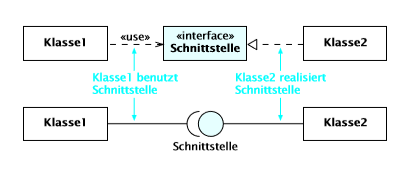
\includegraphics[width=\columnwidth]{Images/schnitstellen}
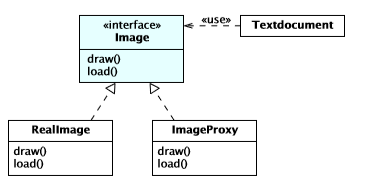
\includegraphics[width=\columnwidth]{Images/schnittstelle_beispiel}

\subsection{Komponenten Diagramm}
\begin{center}
	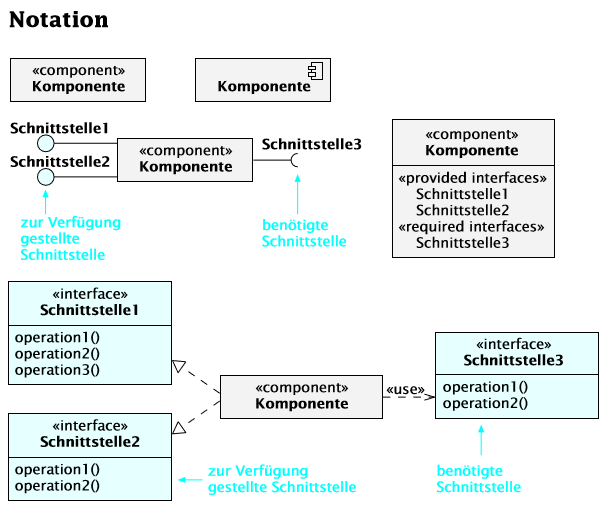
\includegraphics[width=0.9\columnwidth]{Images/komponentdiagramm}
\end{center}

Artefakte enthalten physische Informationen zB Dateien, Executable etc. Abhängigkeiten werden wie folgt definiert:
\begin{center}
	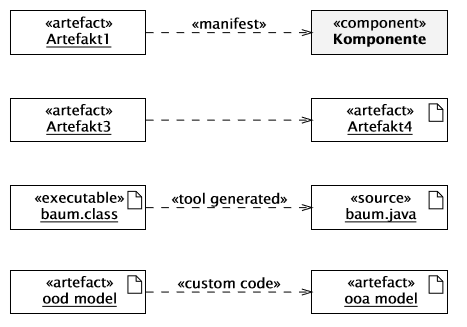
\includegraphics[width=\columnwidth]{Images/artefakte}
\end{center}

